%%%%%%%%%%%%%%%%%%%%%%%%%%%%%%%%%%%%%%%%%%%%%%%%%%%%%%%%%%%%%%%%%%%
%%% Documento LaTeX 																						%%%
%%%%%%%%%%%%%%%%%%%%%%%%%%%%%%%%%%%%%%%%%%%%%%%%%%%%%%%%%%%%%%%%%%%
% Título:		Capítulo 3
% Autor:  	Ignacio Moreno Doblas
% Fecha:  	2014-02-01
% Versión:	0.5.0
%%%%%%%%%%%%%%%%%%%%%%%%%%%%%%%%%%%%%%%%%%%%%%%%%%%%%%%%%%%%%%%%%%%
\chapterbegin{Plan de pruebas y verificación}
\label{chp:App}
\section{Funcionamiento de la aplicación}
    
    Una vez ejecutada la aplicación Android, se nos solicitará la activación de Bluetooth en caso de que este no estuviera previamente activado. Una vez que Bluetooth se encuentra en funcionamiento podemos empezar a escanear dispositivos BLE en el radio de alcance de nuestro teléfono móvil mediante el pulsado del botón en la barra de acción, el cual presenta una imagen con el logotipo de Bluetooth emitiendo señal, tal y como se muestra en la figuras \ref{fig:screen:initialState} y \ref{fig:screen:scanning}.
    
    Al pulsar en el dispositivo encontrado justo después del escaneo, en este caso nuestro pulsómetro comercial adquirido, una nueva actividad aparecerá en pantalla mostrándonos la información relativa al sensor, así como el estado de la conexión, que en un principio será desconectado, tal y como se puede apreciar en la figura  \ref{fig:screen:Desconectado}.  Para conectarnos a él, debemos pulsar en el botón ``Conectar''. Una vez que la conexión GATT cliente-servidor se ha establecido, la interfaz de usuario se actualizará, mostrando los servicios ofrecidos por el sensor, así como las características pertenecientes a cada uno de estos servicios.
    
    \vfill
    
    
\begin{figure}[h] \centering
\begin{minipage}{0.45\textwidth}\centering
    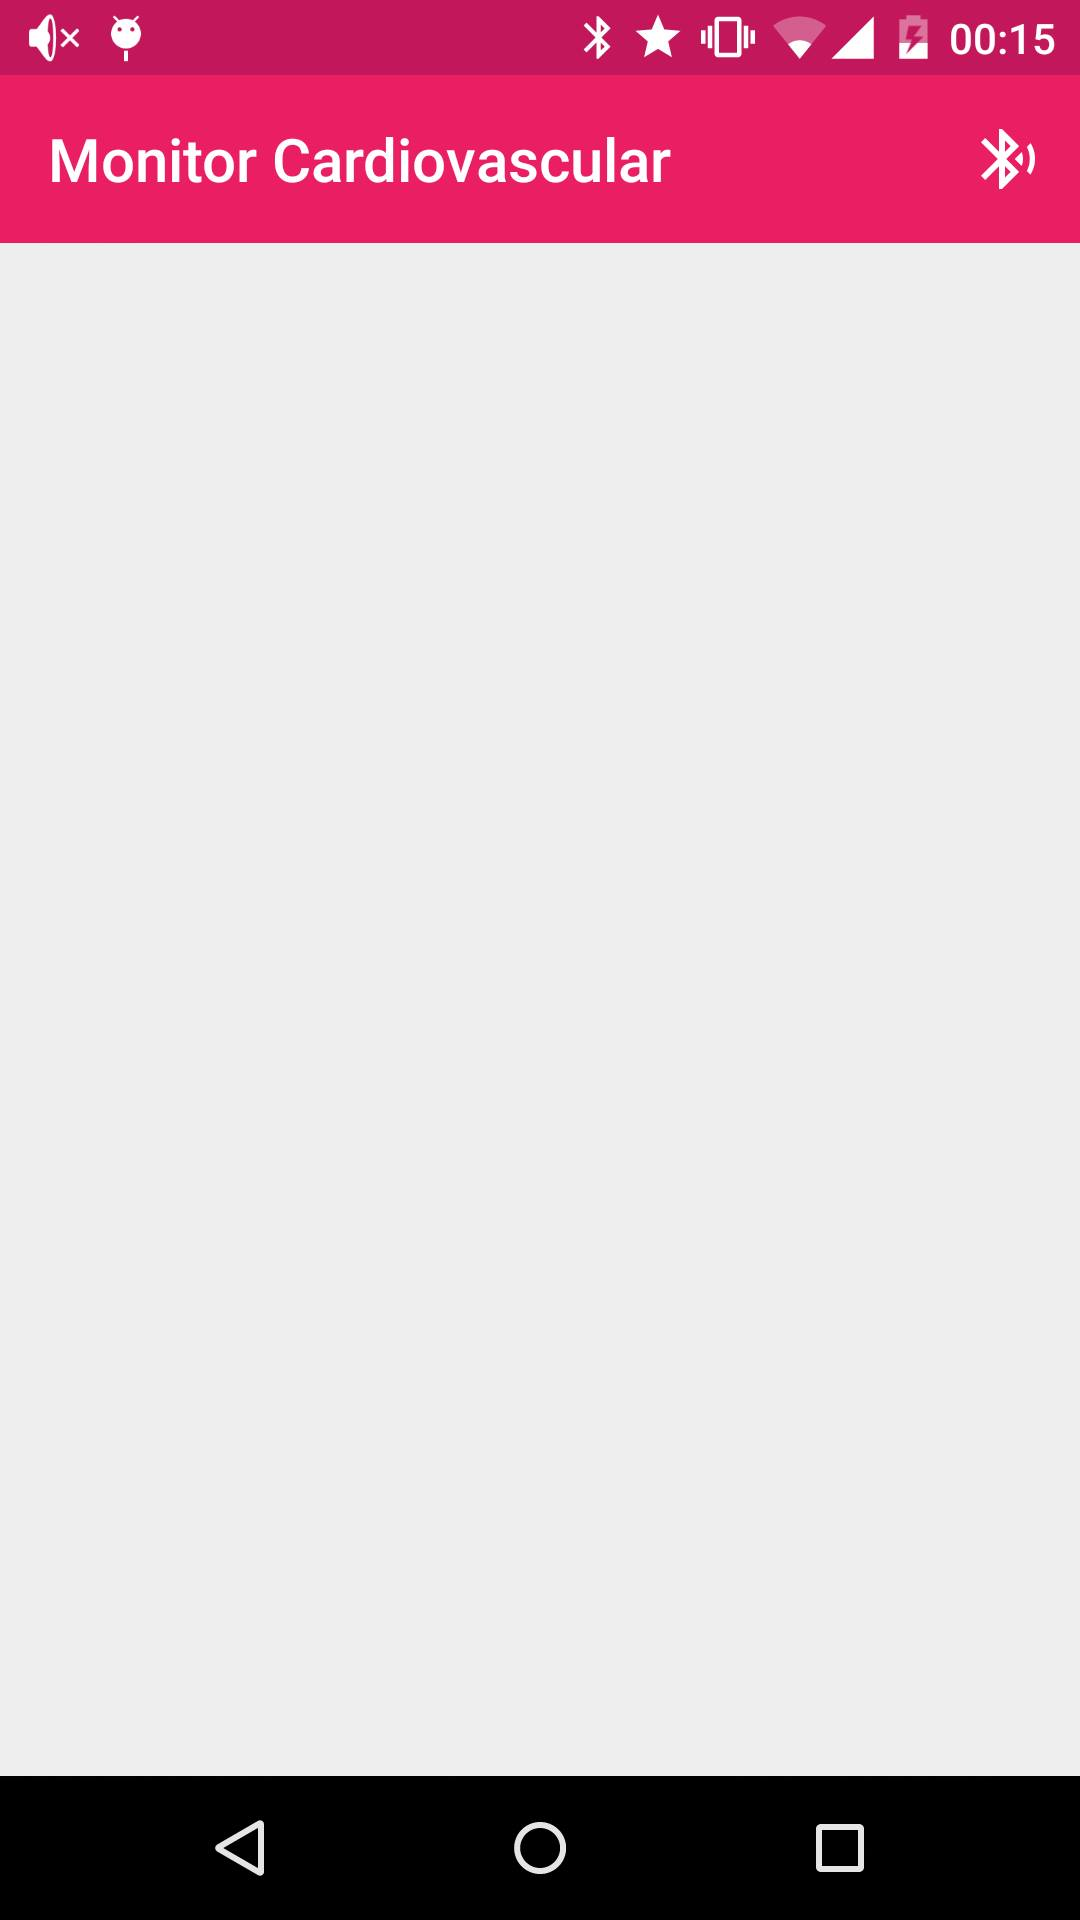
\includegraphics[height=11cm]{graphs/AndroidInicial.png} \caption{Pantalla inicial}\label{fig:screen:initialState}
\end{minipage}
\hfill
 \begin{minipage}{0.45\textwidth}\centering
    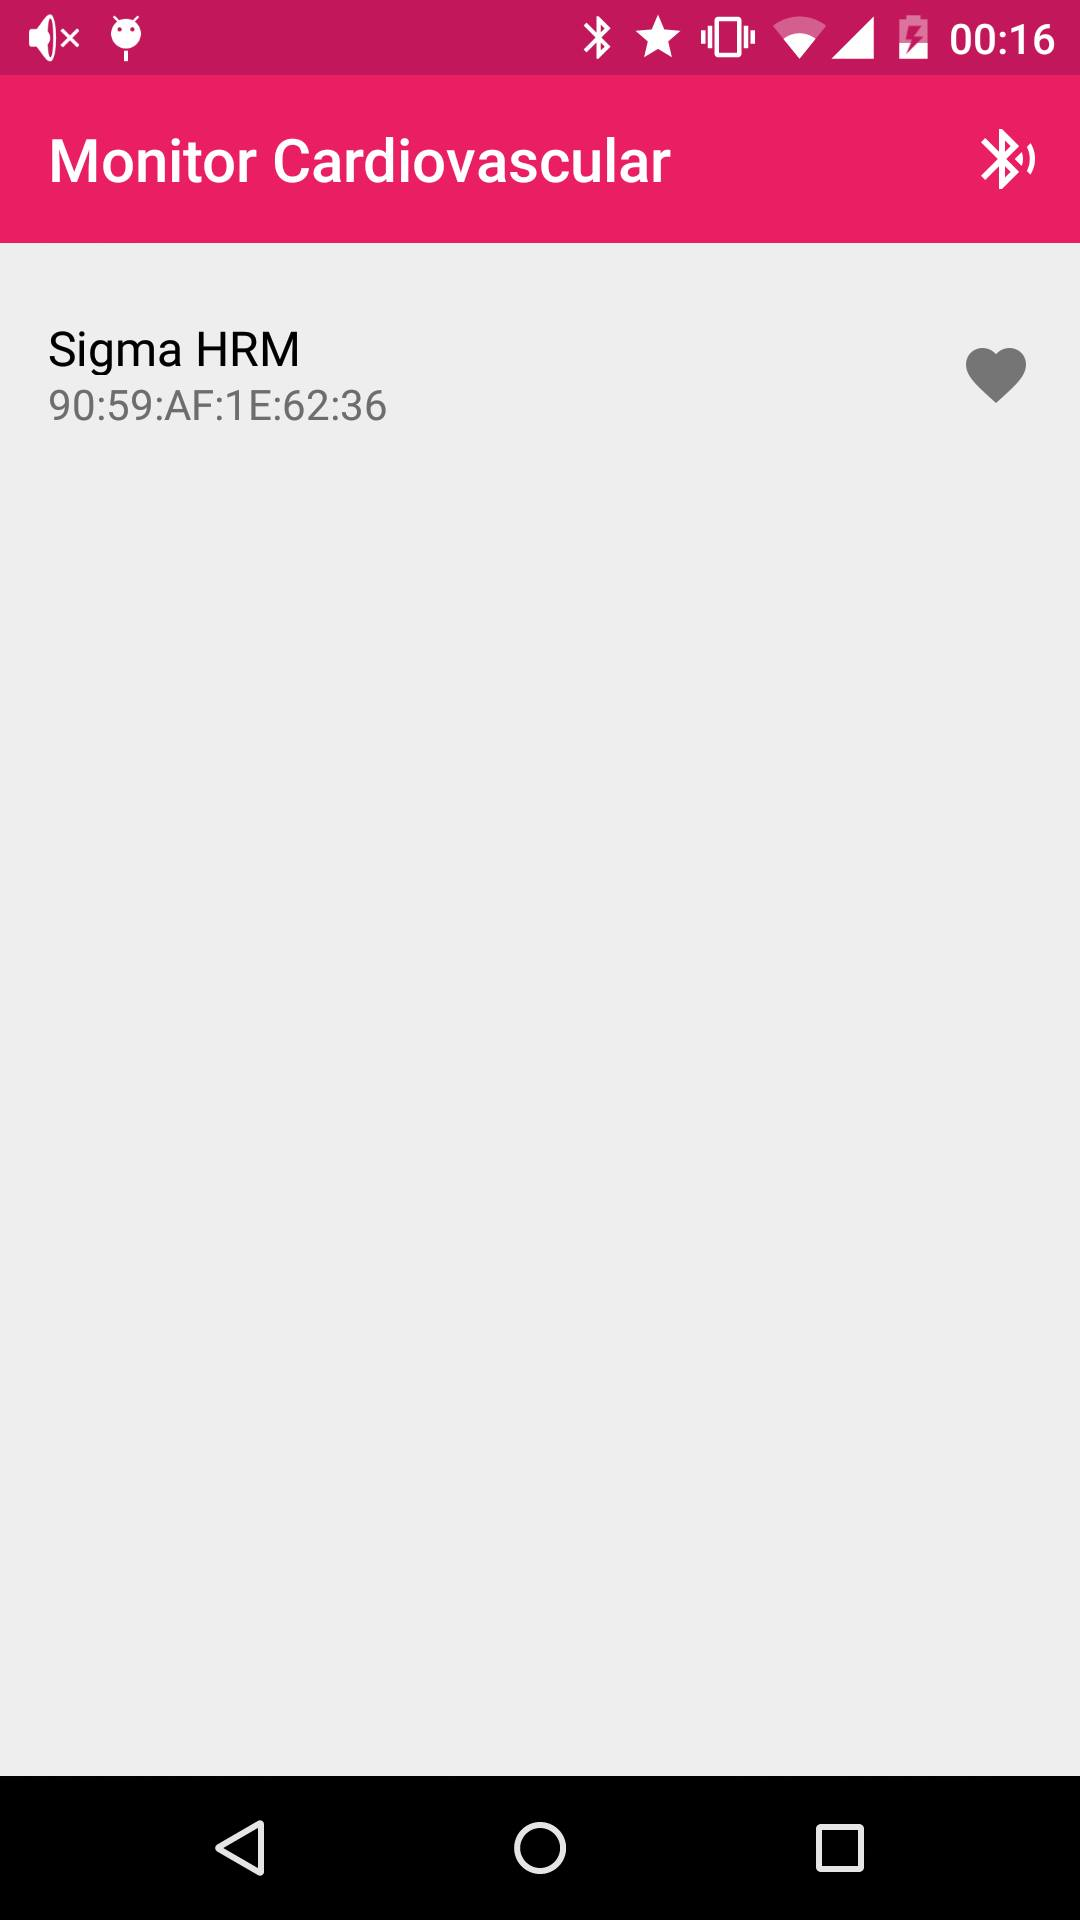
\includegraphics[height=11cm]{graphs/AndroidEscaneo.png} \caption{Dispositivos encontrados}\label{fig:screen:scanning}
\end{minipage}
\end{figure}
    
   En este caso nos encontramos con dos servicios: el servicio ``Servicio Cardiovascular'', que presenta las características ``Medida del ritmo cardíaco'', ``Ubicación del sensor'' y ``Punto de control'' y el servicio ``Servicio de batería'', que presenta una característica que nos permite comprobar el porcentaje de batería restante del pulsómetro. Para empezar a recibir datos de frecuencia cardíaca debemos hacer click en la característica ``Medida del ritmo cardíaco''. Esto activará el cliente HTTP, de forma que enviaremos a nuestro servidor web cada valor que nos llega del pulsómetro. La interfaz de usuario también reflejará cada valor recibido en el campo ``Datos''. La figura \ref{fig:screen:Conectado} muestra dicho proceso.
 
 \begin{figure}[H] \centering
 \begin{minipage}{0.45\textwidth}\centering
    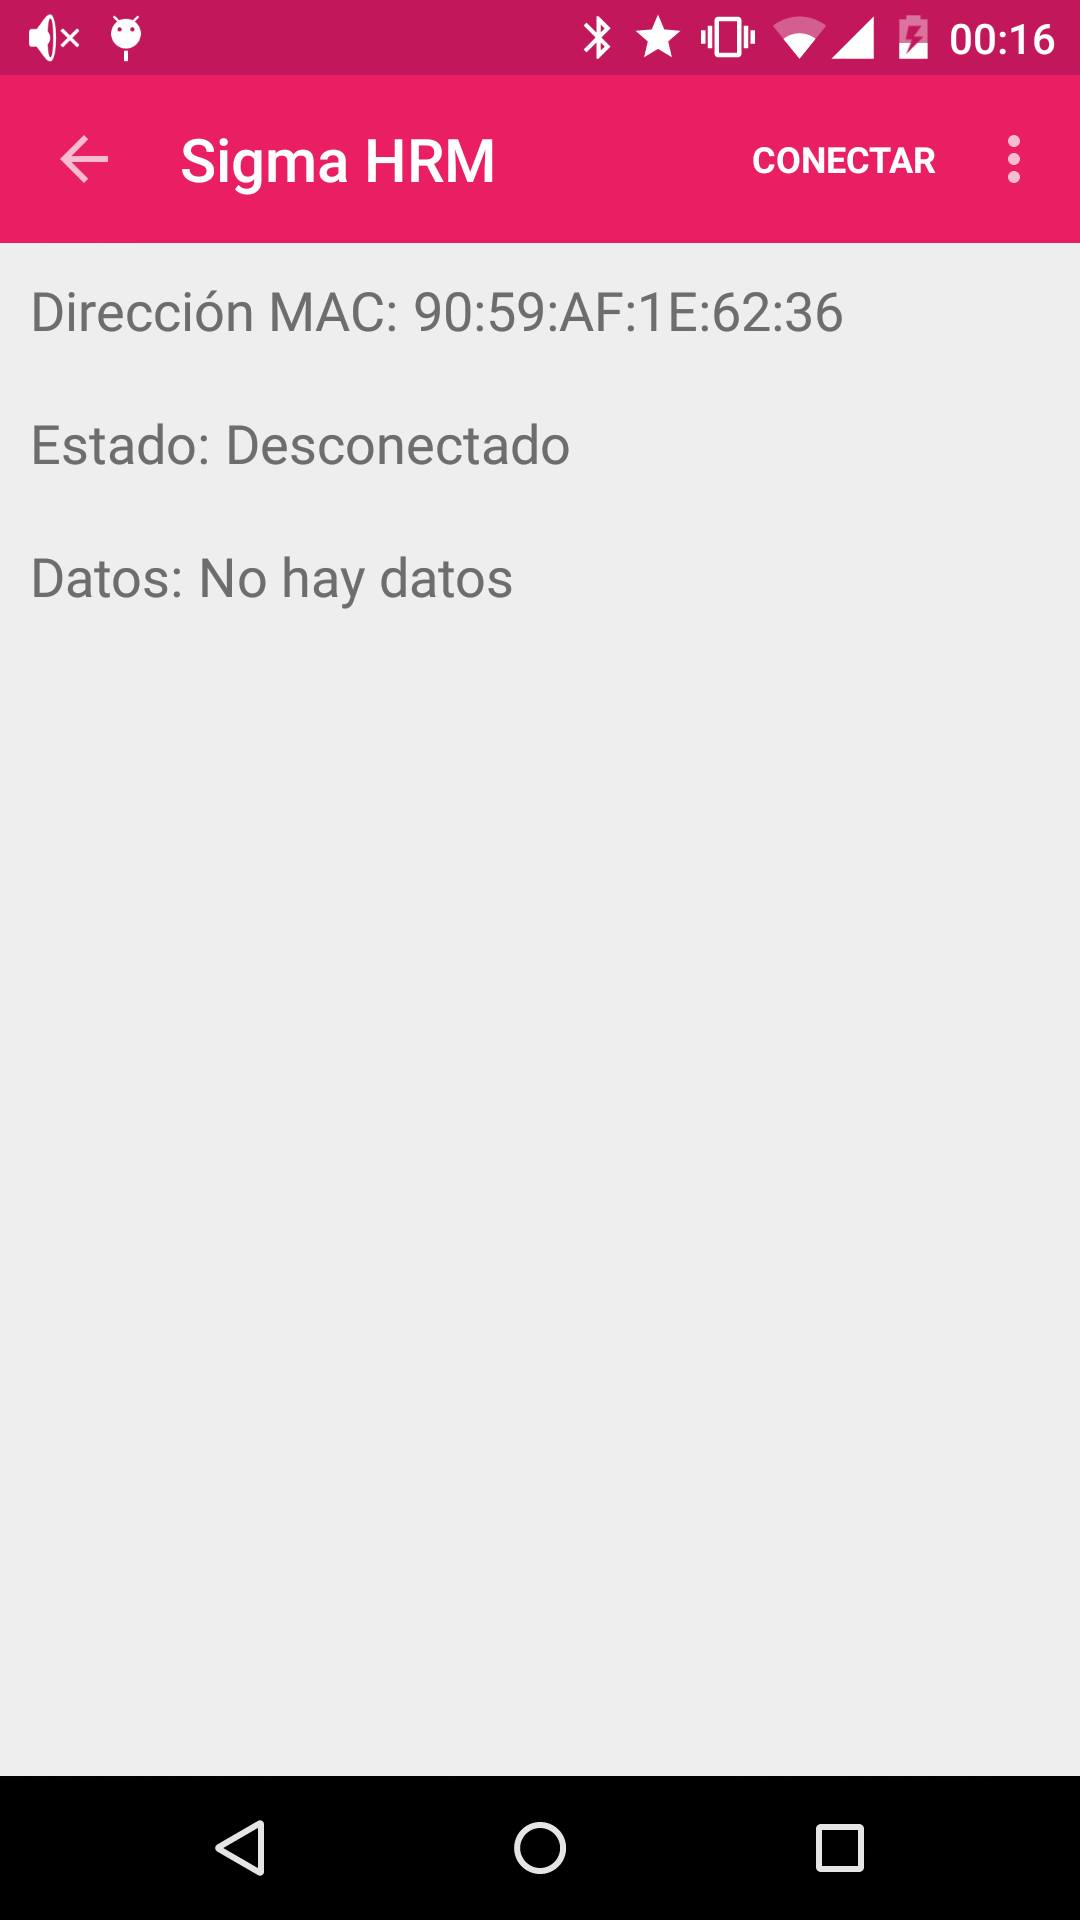
\includegraphics[height=11cm]{graphs/AndroidDesconectado.png} \caption{Conexión GATT sin establecer}\label{fig:screen:Desconectado}
 \end{minipage}
 \hfill
\begin{minipage}{0.45\textwidth}\centering
    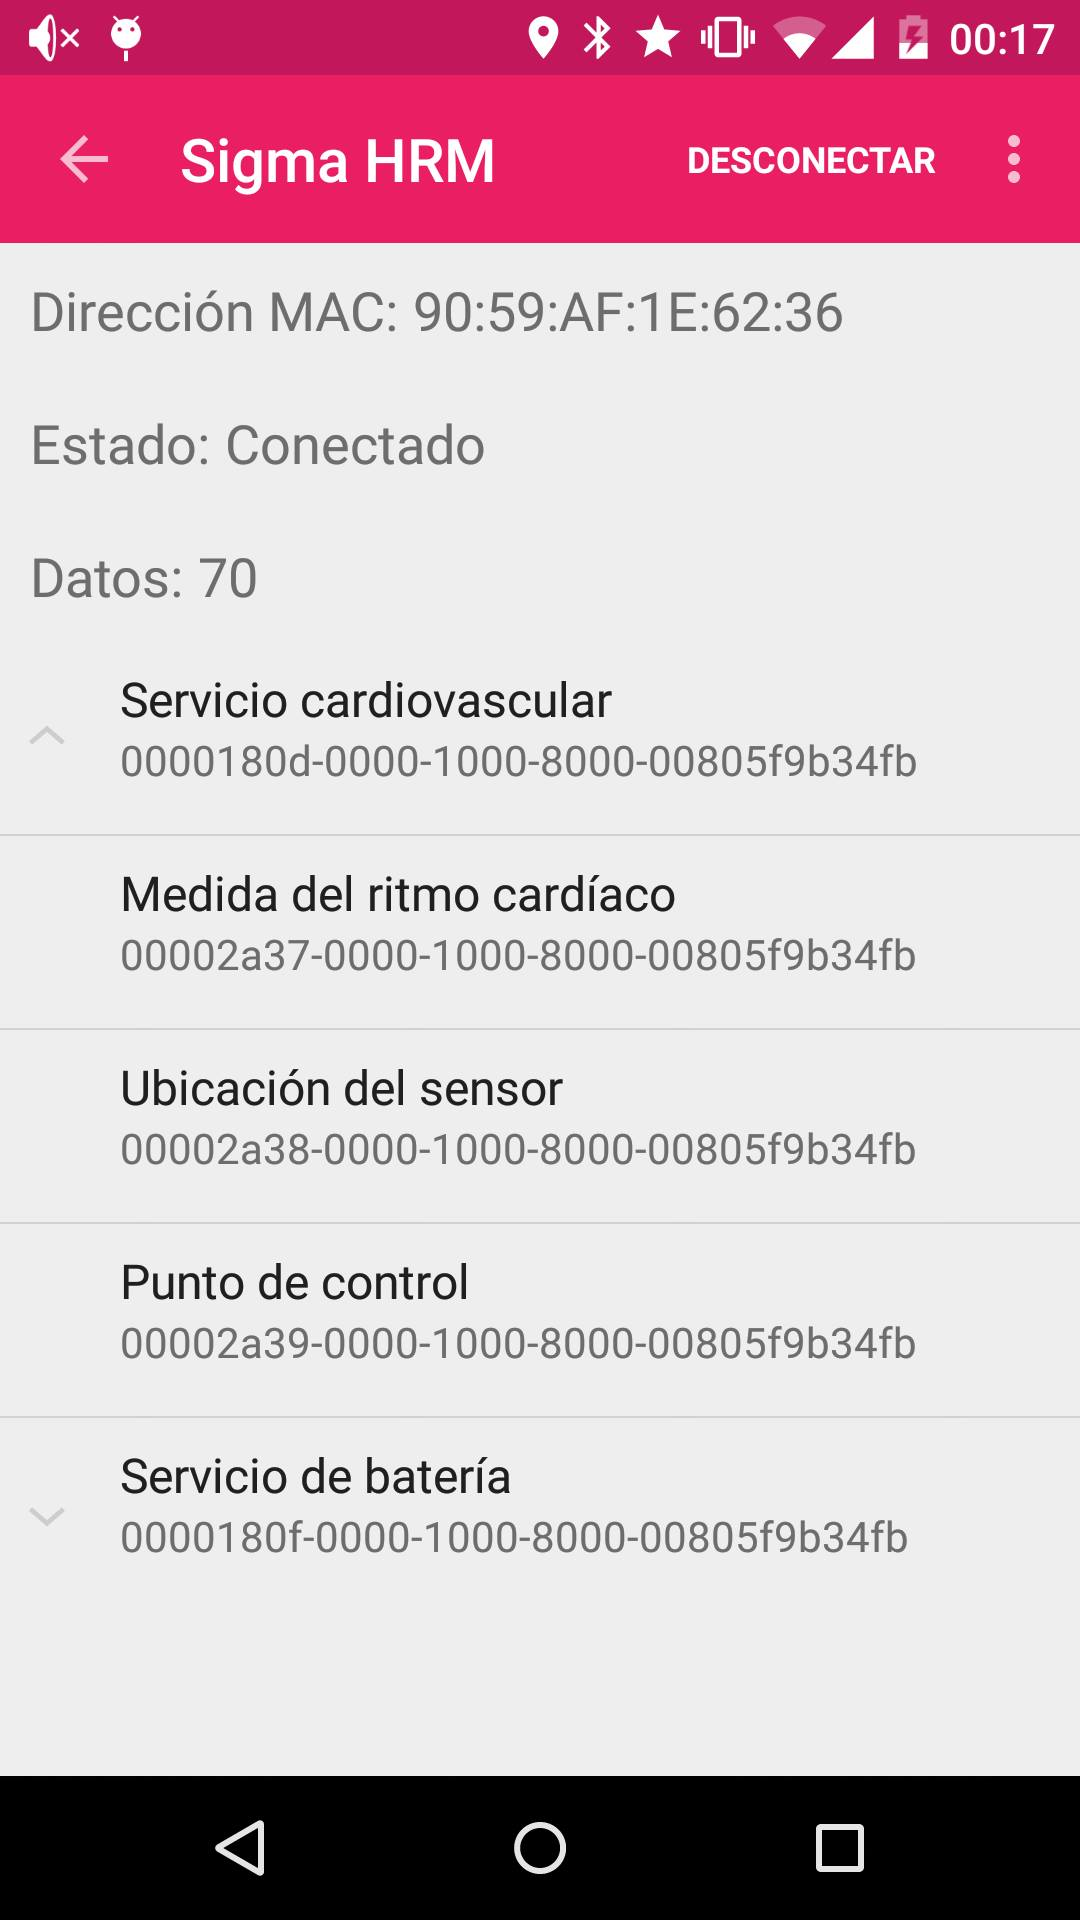
\includegraphics[height=11cm]{graphs/AndroidConectado.png} \caption{Conexión GATT establecida}\label{fig:screen:Conectado}
\end{minipage}
\end{figure}

Es importante mencionar que puesto la conexión GATT cliente-servidor es manejada mediante un servicio en segundo plano, podemos salir de la aplicación y realizar otras actividades, tales como abrir el navegador web o lanzar otras aplicaciones y esto no afectará al comportamiento de la aplicación.
Para desconectarnos del pulsómetro, solo debemos abrir la aplicación de nuevo y pulsar en el botón ``Desconectar''. Esto finalizará el servicio en segundo plano, la conexión GATT y hará que se liberen los recursos usados.

Mientras que estemos desconectados del pulsómetro, nuestro cliente web de monitorización mostrará el estado \tit{Desconectado} en todo momento, tal y como se observa en la figura \ref{fig:web:Desconectado}
    
\begin{figure}[h] \centering
	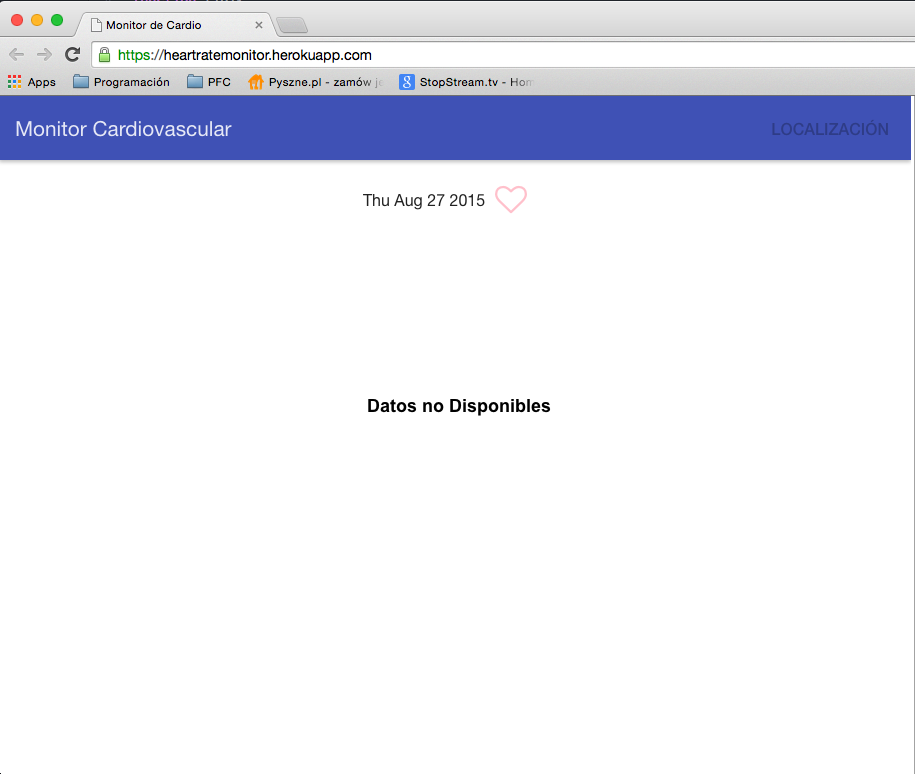
\includegraphics[width=15cm]{graphs/webDesconectado.png} \caption{Cliente web cuando el pulsómetro está desconectado}\label{fig:web:Desconectado}
\end{figure}

En cuanto conectamos con el pulsómetro y seleccionamos la característica de ``Medida del ritmo cardíaco'' en nuestra aplicación Android, los valores empiezan a llegar al servidor web, el cual establece una conexión permanente Web Socket con el cliente web, permitiendo una transmisión en tiempo real de dichos valores. La figura \ref{fig:web:Conectado} representa el cliente web en dicho estado.

\begin{figure}[h] \centering
	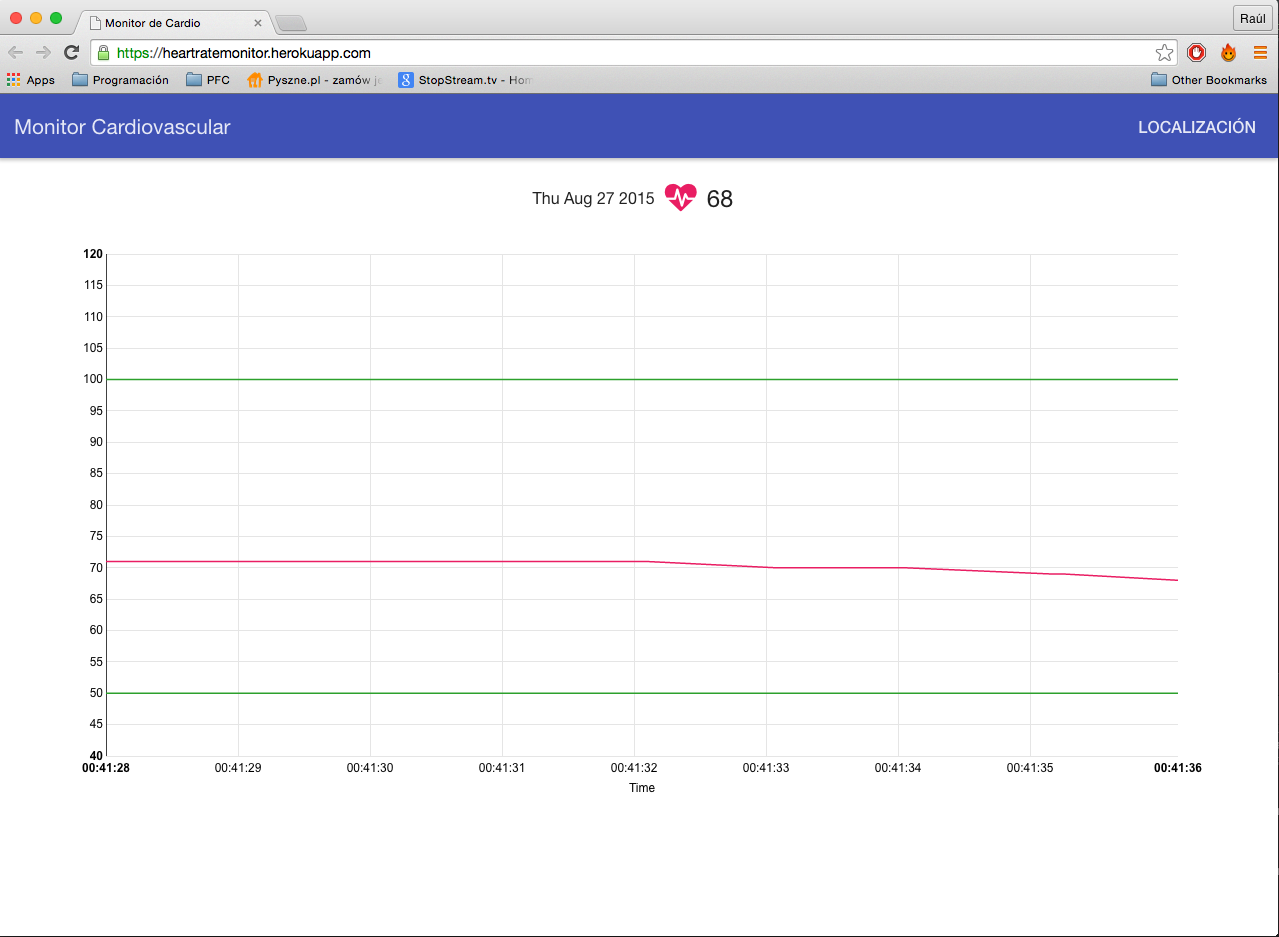
\includegraphics[width=15cm]{graphs/webConectado.png} \caption{Cliente web cuando el pulsómetro está conectado}\label{fig:web:Conectado}
\end{figure}

En la parte superior, justo debajo de la barra de navegación azul, se muestra la fecha actual, un icono representando la palpitación del corazón y el valor actual de frecuencia cardíaca recibido. Justo debajo aparece una gráfica en tiempo real mostrando el valor actual y los últimos valores recibidos con un trazo de color rosa. Las 2 lineas horizontales verdes, las cuales son fijas, delimitan un rango de valores estable (totalmente configurable en función del usuario a monitorizar). Esto está intrínsecamente relacionado con nuestro sistema de notificaciones, ya que se notificará por correo electrónico al usuario encargado de la monitorización siempre que nos topemos con valores fuera de rango, entrando en funcionamiento la lógica explicada en la sección \ref{cap:Servidor}, concretamente en la parte de notificaciones.

Esto se puede apreciar en las figuras \ref{fig:web:Notificaciones} y \ref{fig:web:Reposo}:

\begin{figure}[H] \centering
	\begin{minipage}{0.45\textwidth}\centering
		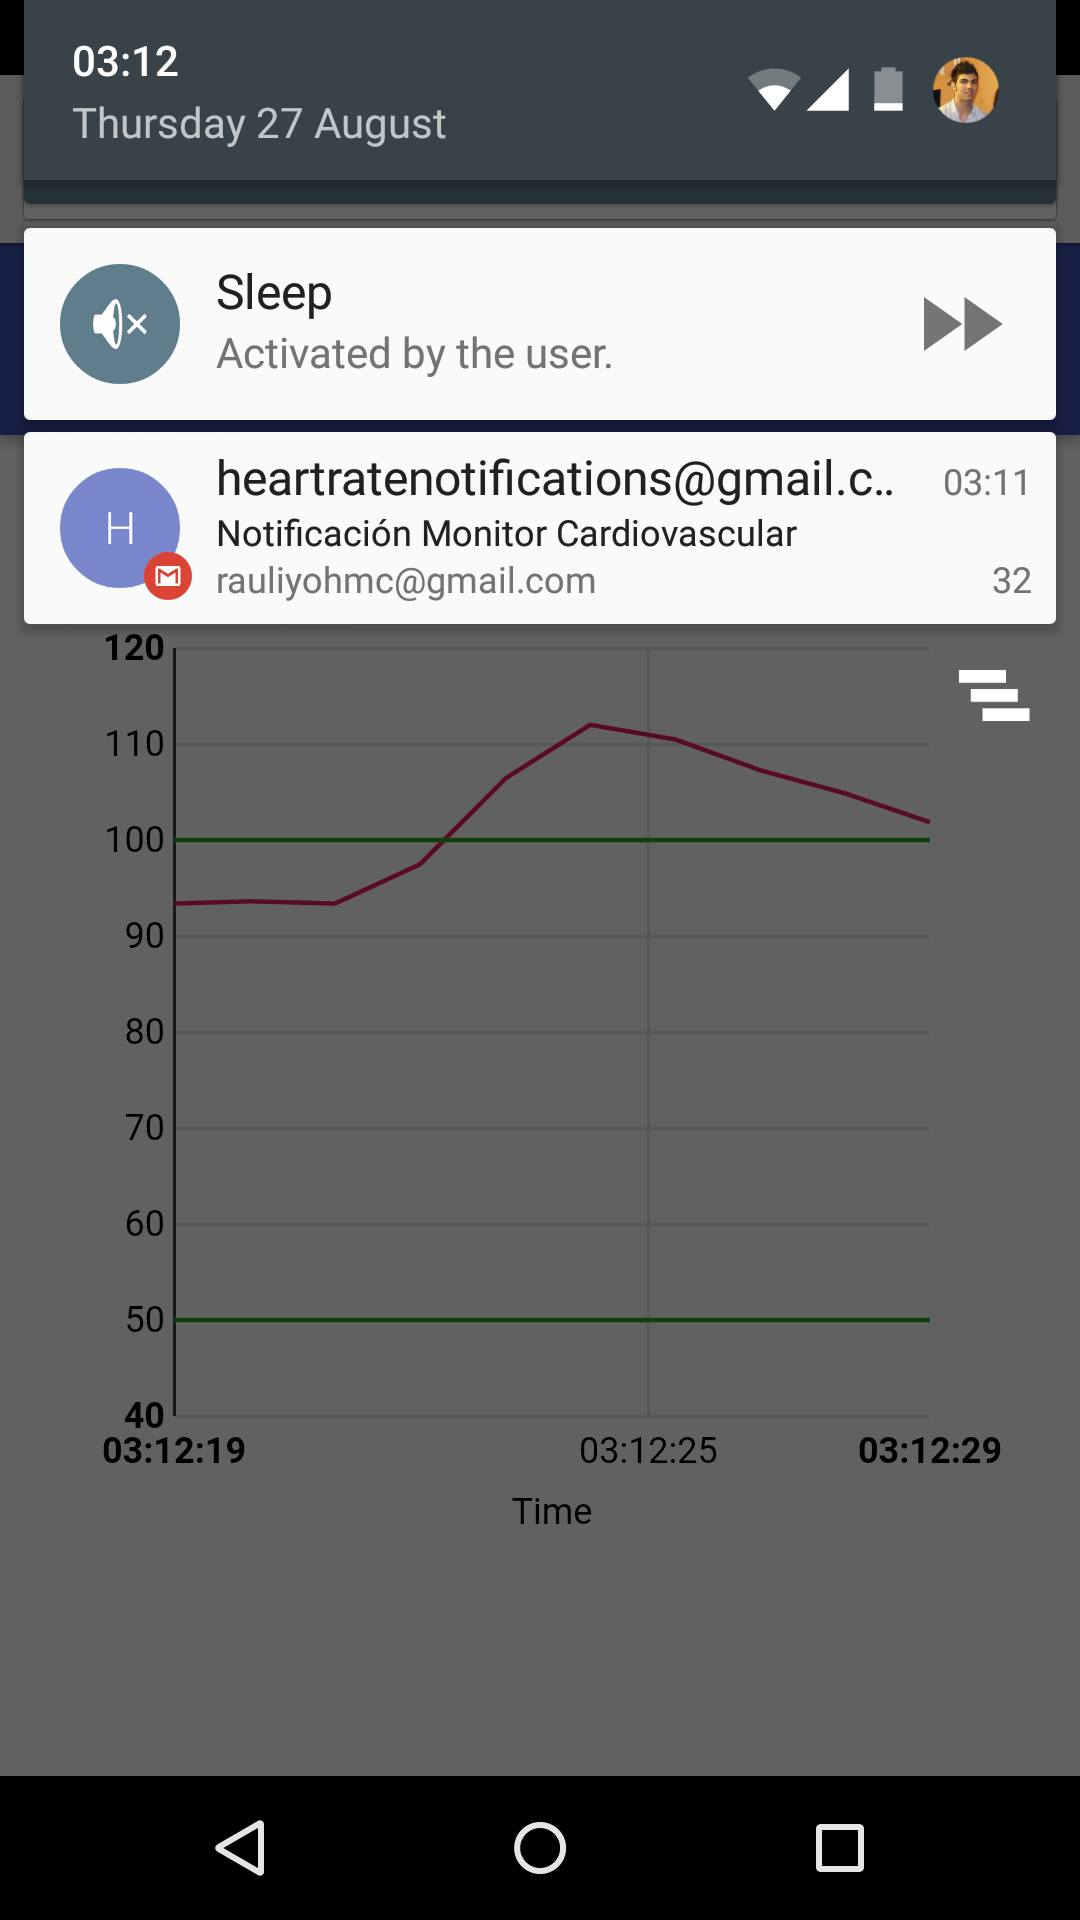
\includegraphics[height=11cm]{graphs/AndroidNotificaciones.png} \caption{Notificación por valor fuera de rango}\label{fig:web:Notificaciones}
	\end{minipage}
	\hfill
	\begin{minipage}{0.45\textwidth}\centering
		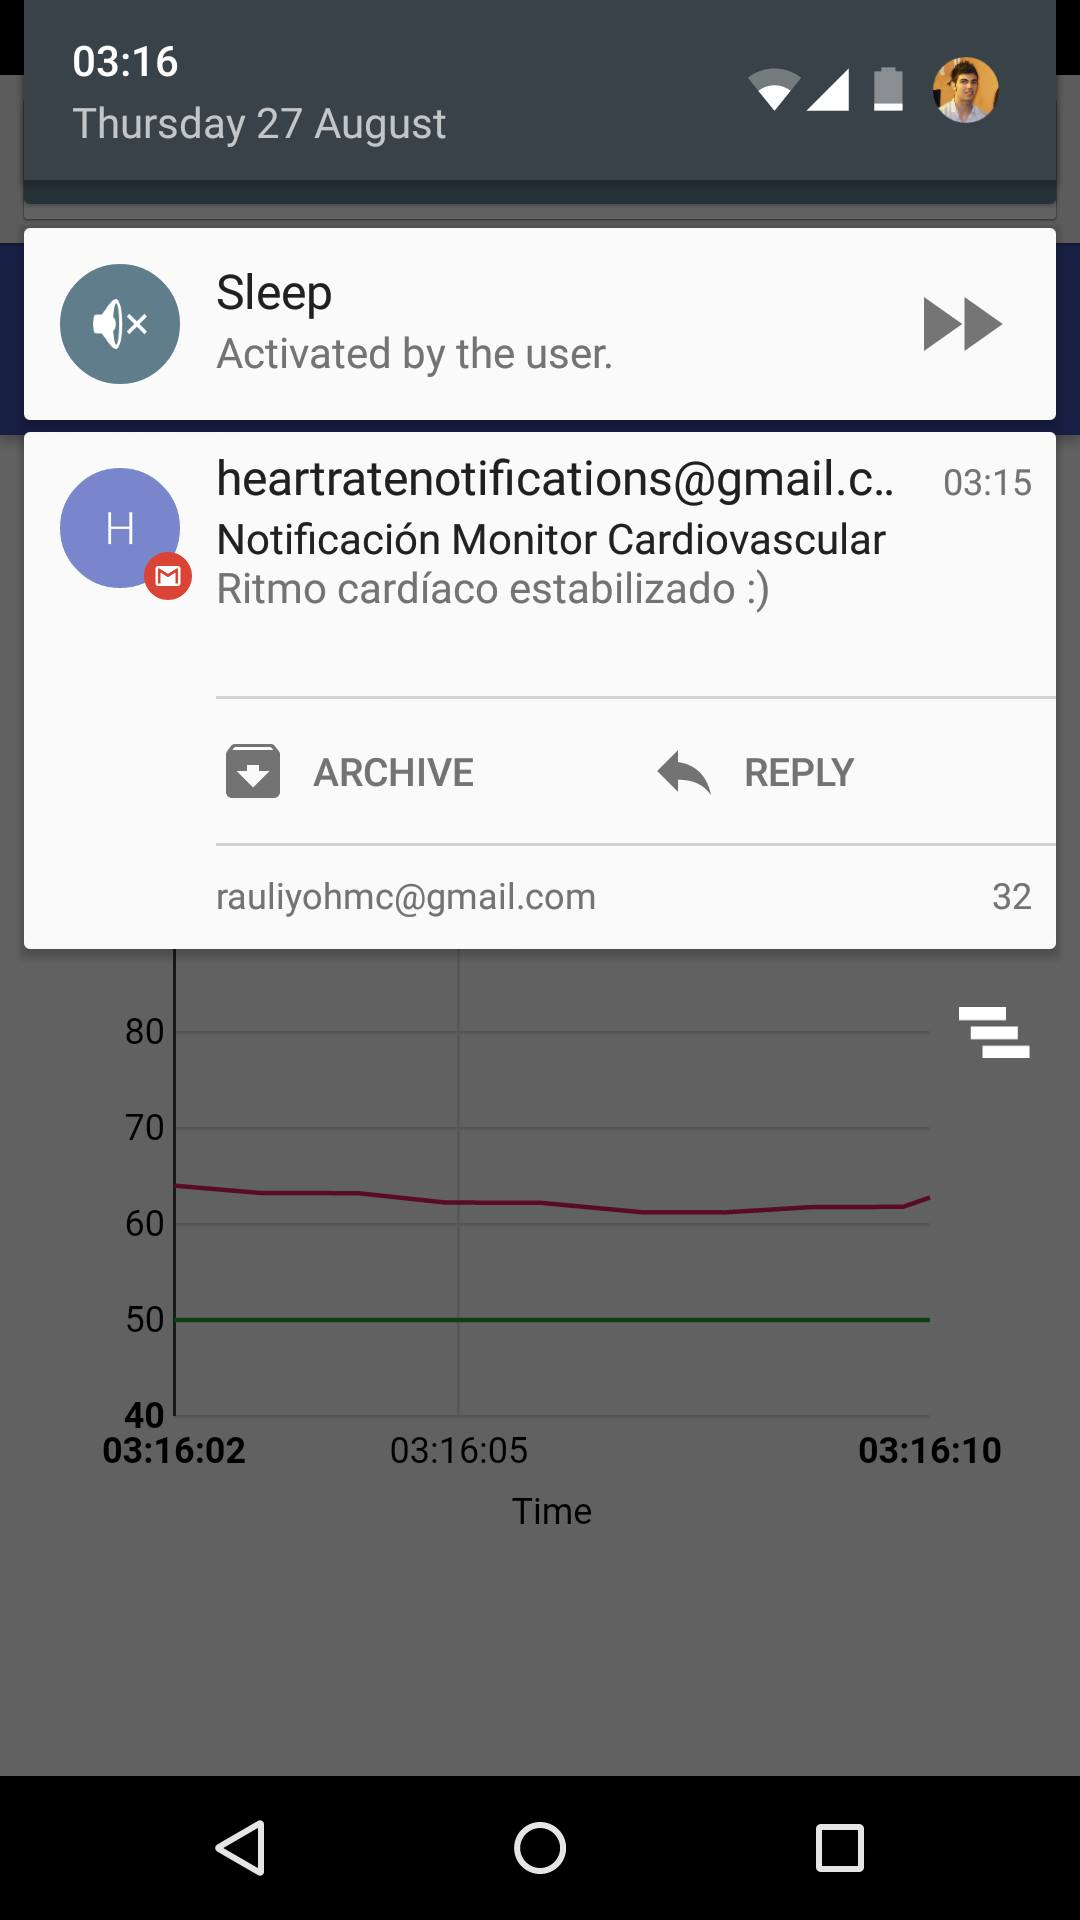
\includegraphics[height=11cm]{graphs/AndroidReposo.png} \caption{Notificación de estabilización}\label{fig:web:Reposo}
	\end{minipage}
\end{figure}

Para consultar la localización exacta del usuario en un determinado instante, debemos de pulsar el botón ``Localización''. Esto nos abrirá automáticamente la aplicación de Mapas de Google, determinando la localización en el mapa, así como la presentación de las coordenadas geográficas, como se puede ver en las figuras \ref{fig:web:Normal} y \ref{fig:web:Mapa}:

\begin{figure}[H] \centering
	\begin{minipage}{0.45\textwidth}\centering
		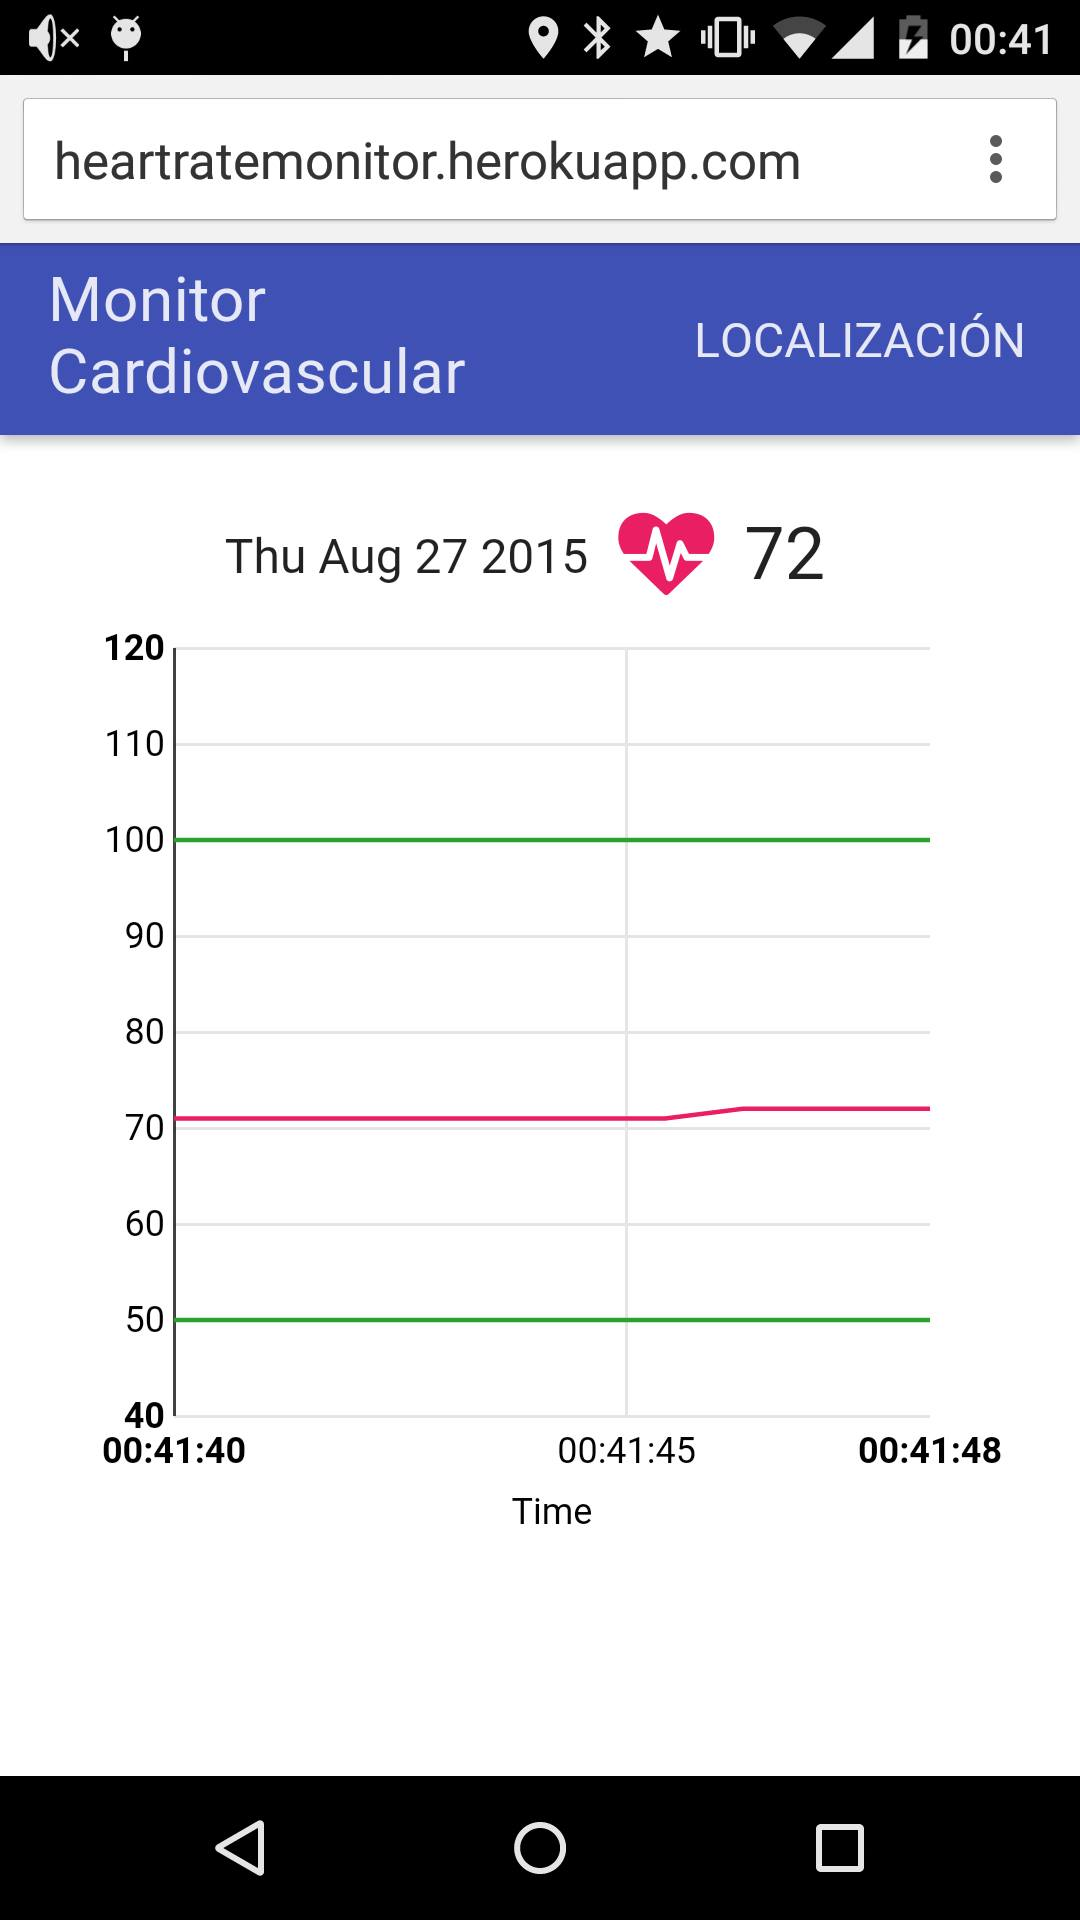
\includegraphics[height=11cm]{graphs/AndroidEmitiendo.png} \caption{Cliente web en un dispositivo móvil}\label{fig:web:Normal}
	\end{minipage}
	\hfill
	\begin{minipage}{0.45\textwidth}\centering
		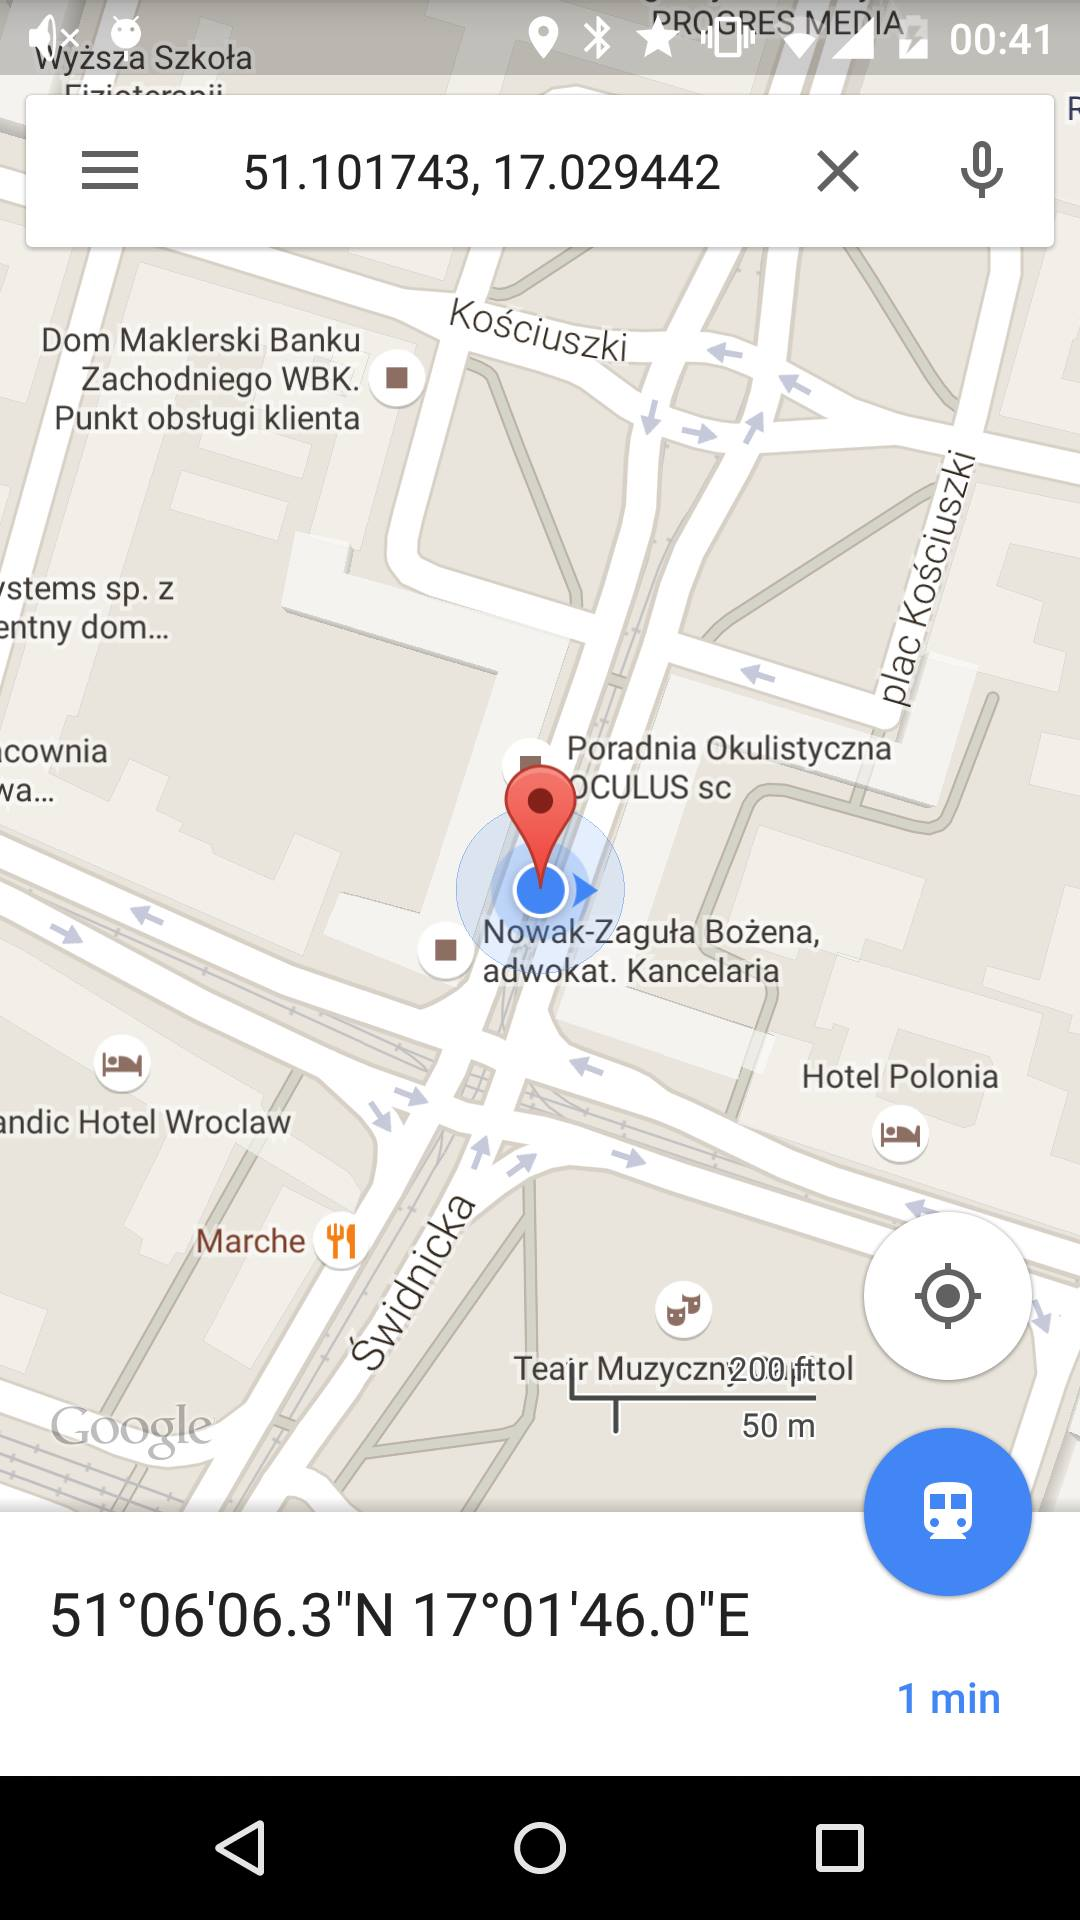
\includegraphics[height=11cm]{graphs/AndroidMapas.png} \caption{Ubicación del usuario en el servicio de mapas de Google}\label{fig:web:Mapa}
	\end{minipage}
\end{figure}

Por último y no menos importante, usamos una base de datos para registrar y guardar cada uno de los valores de frecuencia cardíaca que el servidor web recibe. Para ello hemos recurrido a Mongolab, un servicio de almacenamiento de datos en bases del tipo MongoDB en la nube, el cual nos proporciona de forma gratuita 512 MB de espacio.
La figura \ref{fig:web:dB} muestra un extracto de uno de los documentos almacenados, conteniendo muestras pertenecientes al momento Jueves 27 de Agosto, 3:13 a.m.

\begin{figure}[h] \centering
	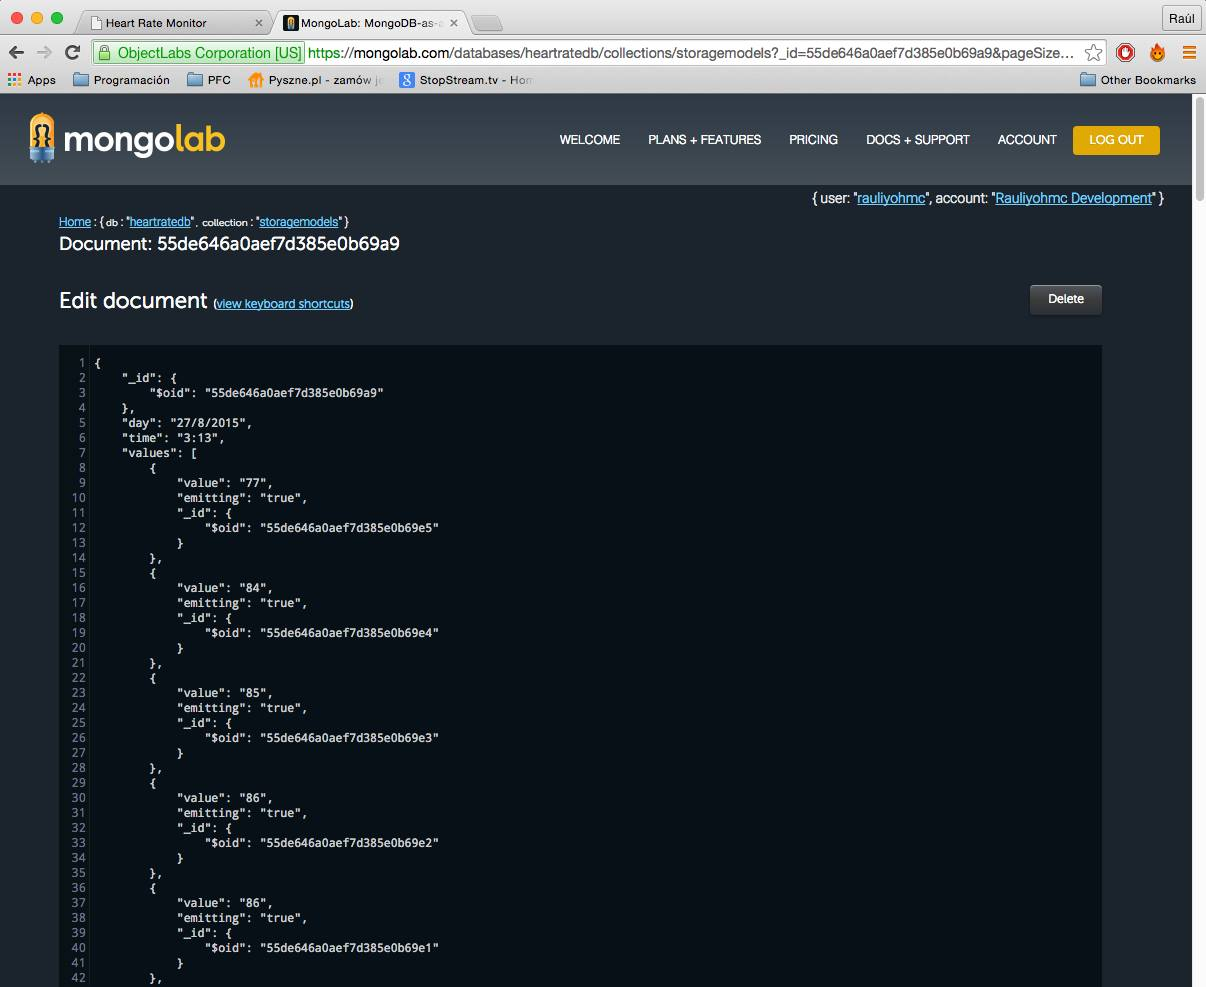
\includegraphics[width=15cm]{graphs/webDB.png} \caption{Servicio de almacenamiento MongoLab en la nube}\label{fig:web:dB}
\end{figure}

\section{Pruebas realizadas}
      
\subsection{Comparación con electrocardiograma}

\begin{figure}[h] \centering
	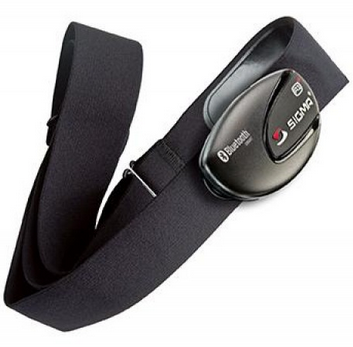
\includegraphics[width=10cm]{graphs/sigma.png} \caption{Sigma R1 Blue Comfortex+}\label{fig:sigma}
\end{figure}

Para cerciorarse de que los valores de frecuencia cardíaca mostrados en la aplicación se ajustan a la realidad, es necesario comparar los valores obtenidos por nuestro pulsómetro pectoral con un aparato de medición calibrado.
Para ello, recurrimos a la ayuda de una doctora ejerciendo en la ciudad de Wroclaw (Polonia), la cual amablemente se ofreció voluntaria para realizar medidas de nivel de frecuencia cardíaca emitidas por un electrocardiograma y así comparar los resultados con las medidas emitidas por el pulsómetro.

El pulsómetro utilizado ha sido el Sigma R1 Blue Comfortex+, el cual se muestra en la figura \ref{fig:sigma}. En el envoltorio podemos observar que afirma tener precisión de ECG (electrocardiograma).

Realizamos el estudio de 3 distintas situaciones, con todos los electrodos del electrocardiógrafo conectados a través del cuerpo y el pulsómetro Sigma comercial atado al pecho mediante su respectiva correa, con los dos electrodos situados en el pecho.
Los resultados obtenidos pueden verse reflejados en la tabla \ref{tab:SAR}:

\begin{table}[H]%
	\centering
	\begin{tabular}{|l|c|c|}
		\hline
		\hline
		\tbf{Actividad}&\tbf{Rango} &\tbf{Error (\%)}\\ \hline 
		\tbf{Reposo} &50-70 bpm& 5.8 \% \\ \hline
		\tbf{Actividad Ligera}& 80-100 bpm& 1.5 \% \\ \hline
		\tbf{Actividad intensa} &  150-170 bpm & 0 \% \\ \hline
		\hline 
	\end{tabular}
	\caption{Tabla de comparacion de mediciones} \label{tab:SAR}
\end{table}

En principio empezamos midiendo el latido del corazón en situación de reposo, mediante una posición estática estando de pie. Se pudo comprobar que existe una pequeña variación en la medida del pulsómetro relativa al electrocardiógrafo profesional, en torno a los +-3/4 bpm (latidos por minuto). Posteriormente empezamos una actividad cardiovascular ligera, alcanzando valores en el rango de las 80-100 pulsaciones por minuto y obtuvimos una mayor precisión, en torno a los +-1/2 bpm. Por último realizamos un trote intenso sobre el sitio hasta alcanzar valores cercanos a las 160 pulsaciones por minuto. De manera sorprendente, las medidas en este caso coincidían plenamente con las proporcionadas por el electrocardiograma.

Concluimos pues con unas medidas bastante exactas en todos los casos, llegando a igualar la medición del electrocardiograma en situaciones de ejercicio intenso. Esto se debe a que, en esencia, el fundamento del pulsómetro comercial de pecho es el mismo que el del electrocardiograma, registrando la actividad eléctrica del corazón que se produce en cada latido cardíaco.

Como contrapartida, existen sensores ópticos del ritmo cardíaco, los cuales funcionan mediante la emisión de luz LED a los capilares, y midiendo la frecuencia de bombeo de la sangre. Estos proveen una precisión alta en situaciones de reposo e inmovilidad, pero no son capaces de medir la frecuencia cardíaca en movimiento. Y en situaciones en las que paramos a medir el latido del corazón después de un intenso ejercicio proveen una precisión bastante baja, con errores en la medida de hasta el 40 \%.

\subsection{Consumo de energía}
Hemos realizado una estimación del consumo de batería medio que nuestra aplicación Android exige. Para ello, hemos usado el dispositivo conectado y emitiendo al servidor durante una hora en reposo, y durante una hora haciendo ejercicio en el exterior. El teléfono móvil utilizado ha sido un Nexus 5.
Durante el periodo en reposo, utilizando conexión inalámbrica a Internet, el teléfono disminuyó su batería un 5 \% en una hora, lo que nos da una estimación de duración de unas 20 horas, siempre que no usemos otras aplicaciones, ya que aquí solo consideramos el consumo del servicio funcionando en segundo plano.
Durante el periodo de ejercicio, y usando la red LTE de un plan de pago, la batería bajó en un 12 \% en una hora, lo que nos da una duración aproximada de 8.5 horas.

Los resultados obtenidos son sorprendentes y nos brindan un sistema capaz de aguantar medio día sin tener que recargar la batería, todo ello considerando todos los recursos utilizados mientras el servicio funciona en segundo plano, que son ni más ni menos el servicio de localización de Google, la conexión GATT cliente-servidor y los envíos de datos al servidor web a través del protocolo HTTP. Este bajo consumo se ve justificado por el hecho de que el protocolo BLE consume muy poca energía. La poca carga de datos que las peticiones HTTP acarrean y el alto intervalo de escaneo del servicio de localización (comprobando cada 2 minutos si existe una nueva posición del usuario) también contribuyen a dicho propósito.

\subsection{Retardo del sistema}
Cuando hablamos de retardo del sistema, nos referimos al tiempo que ha pasado desde que recibimos una nueva muestra de frecuencia cardíaca en nuestra aplicación puente Android, hasta que dicho valor aparece reflejado en la aplicación web. Obviamente esto está influenciado en parte por la velocidad de conexión a Internet en la cual nos encontremos sumergidos. En cualquier caso hoy en día las conexiones que manejamos a diario, ya sea en casa usando una conexión ADSL de alta velocidad, o nos encontremos en la calle usando una conexión HDSPA o LTE proporcionada por el proveedor de servicios contratado nos garantizan un rápido acceso a Internet.

\begin{figure}[h] \centering
	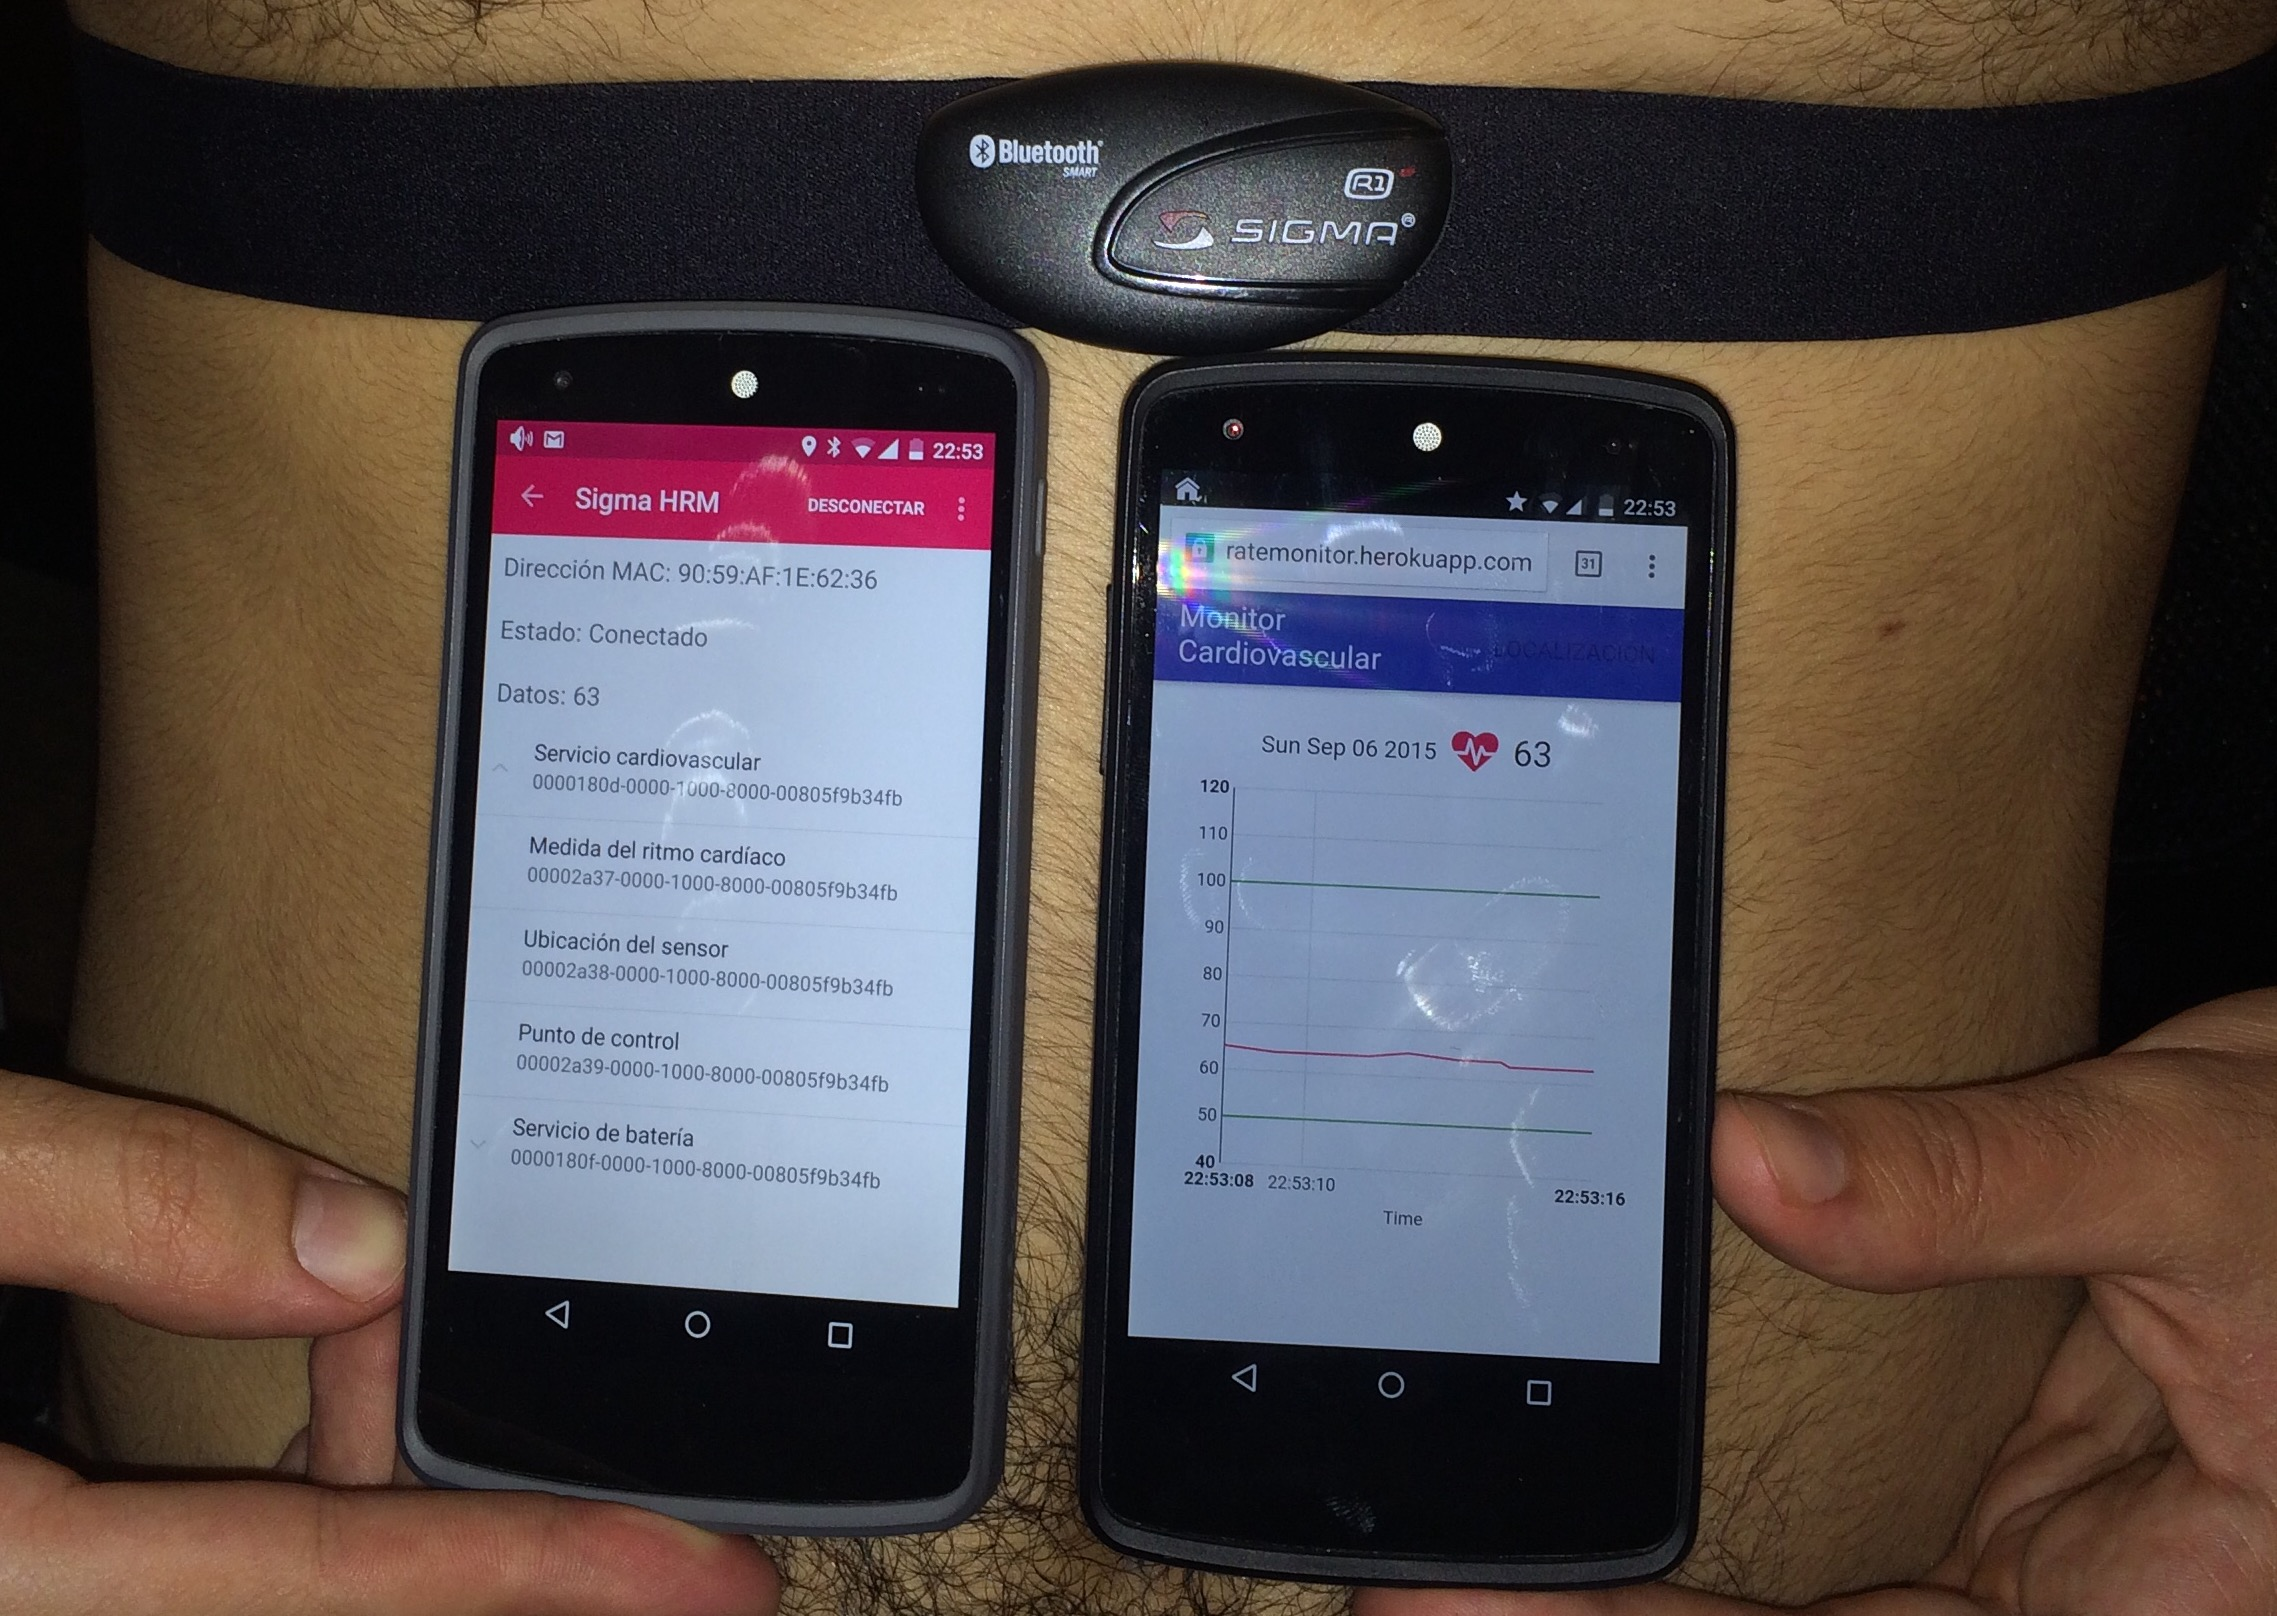
\includegraphics[width=15cm, keepaspectratio]{graphs/FullSizeRender.png} \caption{Captura del sistema en funcionamiento}\label{fig:prueba}
\end{figure}

Hemos puesto nuestro sistema a prueba en el caso extremo para estudiar su viabilidad. Para ello hemos recurrido a Heroku, un servicio gratuito de almacenamiento de aplicaciones web en la nube. El servidor que se nos ha asignado se encuentra en Virginia, Estados Unidos, con lo cual vamos a experimentar una conexión Wroclaw-Virginia-Wroclaw. El primer paso se trata de enviar los datos desde nuestra aplicación Android a nuestro servidor web localizado en Estados Unidos y posteriormente el servidor deberá entregar dichos datos a nuestro navegador web mediante la emisión de eventos utilizando una conexión de tipo socket.

La figura \ref{fig:prueba} muestra una captura tomada durante la realización de la prueba. Como se observa, el móvil de la izquierda muestra la aplicación Android, que recibe la información del pulsómetro y la envía al servidor, mientras que el móvil de la derecha es el que muestra la información proporcionada por el servidor en el navegador web, pudiéndose ver como los valores de pulsación coinciden.

Los resultados son asombrosos, es prácticamente imposible apreciar un retraso desde que la aplicación Android muestra el valor recibido en el campo de datos, hasta que este se ve reflejado en la web. Podríamos estimar un retardo en torno a los 100 milisegundos siendo algo conservadores, con lo cual se cumple con creces el objetivo de simulación de tiempo real del sistema.

Para finalizar, hemos incluido un resumen de las pruebas realizadas en la figura \ref{table:pruebas}.

\begin{figure}[h] \centering
	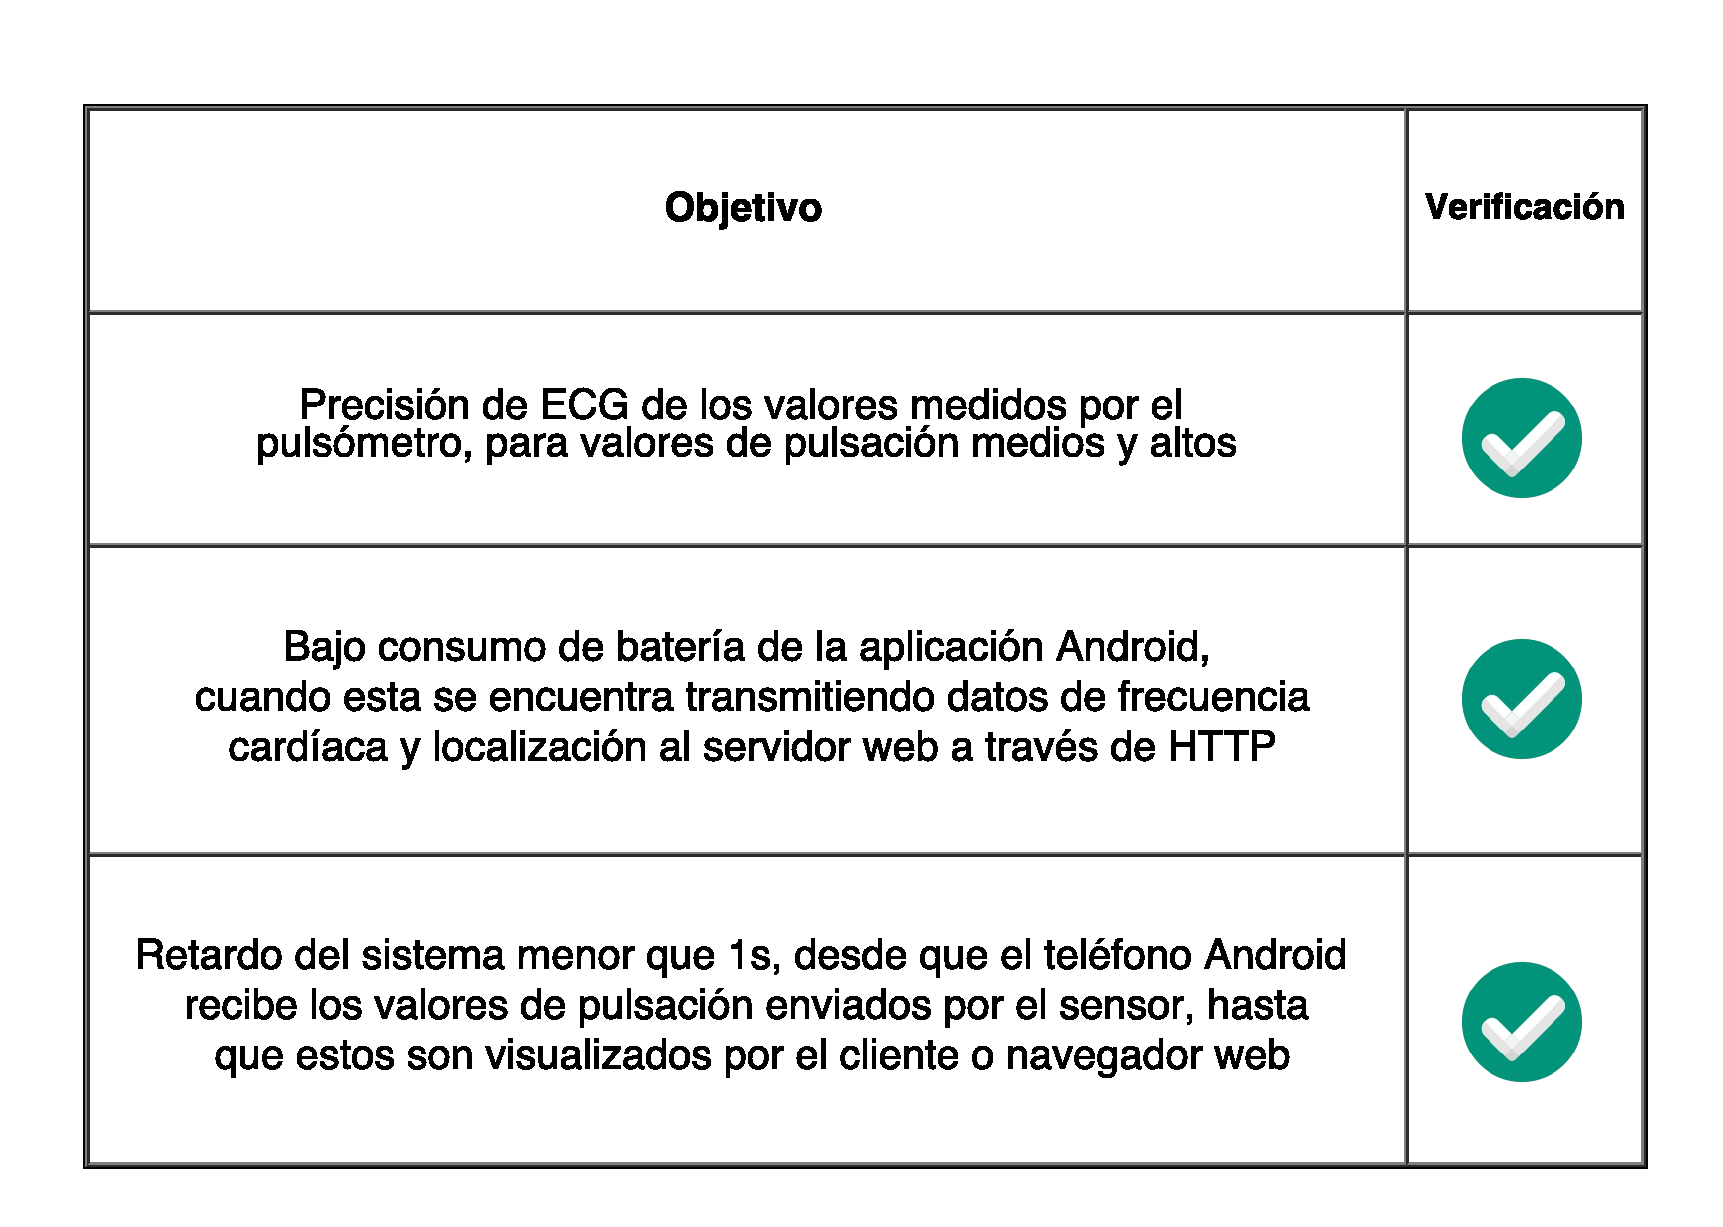
\includegraphics[width=15cm]{graphs/resumenObjetivos.pdf} \caption{Resumen de las pruebas realizadas}
	\label{table:pruebas}
\end{figure}
 
\section{Realización de los objetivos}

\subsection{Aplicación Android}

\subsubsection{Capacidad de detectar sensores BLE próximos al dispositivo}
    La aplicación cumple con el objetivo de ser capaz de escanear sensores con pila de reloj que usan el protocolo BLE para emitir información, ya sean monitores de frecuencia cardíaca u otra orientación médica, emisores de publicidad, etcétera.

\subsubsection{Capacidad de conectarse a cualquier sensor BLE registrado}
    La aplicación permite conectarnos a cualquiera de ellos para así consultar los servicios GATT ofrecidos, junto con cada una de sus características GATT, tal y como se observa en la figura \ref{fig:screen:Conectado}.

\subsubsection{Capacidad de leer características GATT ofrecidas por el sensor}
    La aplicación es capaz de leer el valor contenido en una cierta característica GATT, mediante la interpretación interna de sus descriptores, proporcionando un valor legible para el ser humano, como puede ser el valor de frecuencia cardíaca (mostrado en el campo ``datos'' de la figura \ref{fig:screen:Conectado}), la posición del sensor en el cuerpo, o el porcentaje de batería restante del sensor.
    
\subsubsection{Capacidad de enviar los parámetros relevantes a través del protocolo HTTP a nuestro servidor web}
   La aplicación cumple con el objetivo de enviar al servidor web los valores de ritmo cardíaco y localización obtenidos a través de los servicios que corren en segundo plano.
    
\subsection{Aplicación web}

\subsubsection{Capacidad de determinar si el sensor está conectado al sistema}
	La aplicación cumple con el objetivo de reflejar en todo momento el estado de la conexión del sensor. El estado desconectado se manifiesta mediante la iconografía de un corazón hueco y mediante la ausencia de gráfica en el centro de la pantalla, tal y como se aprecia en la figura \ref{fig:web:Desconectado}. El estado conectado se representa mediante la iconografía de un corazón palpitando.
	
\subsubsection{Capacidad de mostrar la frecuencia cardíaca actual en tiempo real}
	La aplicación es capaz de mostrar el valor de frecuencia cardíaca en tiempo real, mediante la indicación numérica justo a la derecha del icono de corazón latiendo, tal y como se aprecia en la figura \ref{fig:web:Conectado}.
	
\subsubsection{Capacidad de mostrar la evolución de la frecuencia cardíaca mediante el uso de una gráfica dinámica}
	La aplicación cumple con el objetivo de dibujar los valores que van llegando en una gráfica dinámica, la cual mostrará el valor actual junto con los más recientes (cuyo número dependerá del tamaño de la pantalla). Esta gráfica simula un comportamiento en tiempo real, desplazando valores a la izquierda conforme nuevos valores llegan. También presenta dos trazos horizontales configurables representando unos posibles límites dañinos o peligrosos.

\subsubsection{Capacidad de guardar los datos de frecuencia cardíaca en una base de datos}
	La aplicación es capaz de guardar en una base de datos todo registro de frecuencia cardíaca recibido, ordenándolos en documentos de 60 muestras cada uno, representando aproximadamente un minuto de actividad. Esto permitirá un fácil acceso o consulta mediante la indicación del minuto exacto como clave de acceso, así como el día en cuestión.
	
\subsubsection{Capacidad de determinar la posición del usuario usando el servicio de mapas de Google}
	La aplicación cumple con el objetivo de ser capaz de determinar la posición absoluta del dispositivo móvil, gracias al servicio de mapas de Google, tal y como se puede observar en la figura \ref{fig:web:Mapa}. El punto azul representa dicha posición.
	
\subsubsection{Capacidad de notificar por e-mail a un grupo de usuarios interesados en realizar tareas de monitorización}
	La aplicación cumple con las expectativas de notificar al usuario en caso de valores fuera de rango, mediante el envío instantáneo de correos electrónicos, los cuales informarán en todo momento de la evolución de la situación hasta que se detecte una estabilización de los valores, lo que conllevará el fin del periodo de notificaciones a través de una notificación final informativa. En dichos correos también se adjuntará la localización del usuario. Esto se ve reflejado en las figuras \ref{fig:web:Notificaciones} y \ref{fig:web:Reposo}.

\subsubsection{Capacidad de adaptarse fácilmente a pantallas más pequeñas, tales como teléfonos móviles y tabletas}
	La aplicación cumple con el objetivo de adaptarse también a dispositivos móviles, los cuales presentan pantallas más pequeñas, siendo capaz de mostrar información con la misma calidad que si nos encontrásemos en un ordenador personal, sin forzar al usuario a enfocar la pantalla mediante un aumento. Esto se aprecia perfectamente en la figura \ref{fig:web:Reposo}.
	
\chapterend{}